\documentclass[aspectratio=169]{beamer}

\usepackage{listings}
\usepackage{xcolor}

\definecolor{codegray}{rgb}{0.5,0.5,0.5}
\definecolor{codepurple}{rgb}{0.58,0,0.82}
\definecolor{backcolour}{rgb}{0.95,0.95,0.92}

\lstdefinestyle{customc}{
  backgroundcolor=\color{backcolour},
  commentstyle=\color{codegray}\itshape,
  keywordstyle=\color{blue}\bfseries,
  numberstyle=\tiny\color{gray},
  stringstyle=\color{codepurple},
  basicstyle=\ttfamily\footnotesize,
  breakatwhitespace=false,
  breaklines=true,
  captionpos=b,
  keepspaces=true,
  numbers=left,
  numbersep=5pt,
  showspaces=false,
  showstringspaces=false,
  showtabs=false,
  tabsize=2,
  frame=single,
  language=C++
}

\lstset{style=customc}

\usepackage[spanish]{babel}
\usepackage[utf8]{inputenc}
\usepackage[T1]{fontenc}
\usepackage{lmodern}
\usepackage{amsmath, amsfonts}
\usepackage{hyperref}
\usepackage{graphicx}

\usetheme{Madrid}

\title{Introducción a los grafos}
\author{Sebastian Mestre}
\date{}

\begin{document}

\begin{frame}
  \titlepage
\end{frame}

%------------------------------------------------------------
\section{Introducción}

\begin{frame}{¿Qué es un grafo?}
  \begin{itemize}
    \item Un \textbf{grafo} (V,E) tiene conjuntos V de \textbf{vértices} (o nodos) y E de \textbf{aristas} que los conectan.
    \item Nos permite modelar relaciones binarias: ``está conectado con'', ``hay una ruta entre'', etc.
    \item Super general: muchas cosas se pueden ver como casos particulares de grafos.
  \end{itemize}
  \begin{center}
    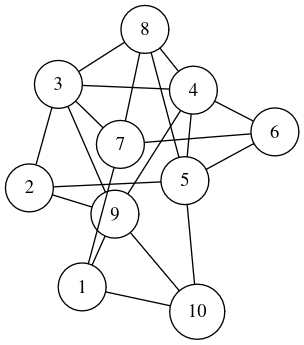
\includegraphics[width=0.33\linewidth]{img/ejemplo1.png}
  \end{center}
\end{frame}

\begin{frame}{Aplicaciones clásicas}
  \begin{itemize}
    \item Detectar partes de una red que estén \textbf{desconectadas}.
    \item Encontrar \textbf{caminos más cortos} en mapas (por ejemplo, rutas de GPS).
    \item Modelar \textbf{redes} de todo tipo: rutas aéreas, internet, redes sociales, etc.
    \item Resolver problemas clásicos como los \textbf{puentes de Königsberg}, que motivaron la teoría de grafos.
  \end{itemize}
  \begin{center}
    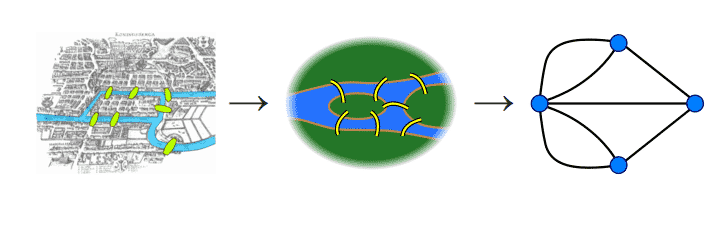
\includegraphics[width=0.5\linewidth]{img/konisberg.png}
  \end{center}
\end{frame}

%------------------------------------------------------------
\section{Conceptos básicos}

\begin{frame}{Grafos dirigidos y no dirigidos}
  \begin{itemize}
    \item \textbf{Grafo dirigido} (dígrafo):
      \begin{itemize}
        \item Las aristas tienen dirección: de un nodo \(u\) hacia un nodo \(v\).
        \item Una arista de \(u\) a \(v\) \textbf{no} implica una de \(v\) a \(u\).
      \end{itemize}
    \item \textbf{Grafo no dirigido}:
      \begin{itemize}
        \item Las aristas no tienen dirección, la conexión es simétrica.
        \item Usando la notación \((u, v)\) se entiende que también existe \((v, u)\).
      \end{itemize}
  \end{itemize}
\end{frame}

\begin{frame}{Caminos y ciclos}
  \begin{itemize}
    \item Un \textbf{camino} es una secuencia de vértices \( v_0, v_1, \dots, v_k \) tal que para cada \(i\) existe una arista entre \(v_i\) y \(v_{i+1}\).
    \item Un \textbf{camino simple} es un camino donde no se repite ningún vértice.
    \item Un \textbf{ciclo simple} es un camino que repite solamente el primero y último, que son iguales.
    \item Si existe un camino entre dos vértices, decimos que \textbf{están conectados} o \textbf{son conexos}.
    \item La \textbf{distancia} entre dos nodos es la longitud (número de aristas) del camino más corto que los conecta. (no definida para nodos no-conexos)
    \item En un grafo no dirigido, una \textbf{componente conexa} es un conjunto de vértices tal que:
      \begin{itemize}
        \item Cualquier par de vértices del conjunto está conectado por algún camino.
        \item Ningún vértice fuera del conjunto está conectado con los de adentro.
      \end{itemize}
  \end{itemize}
\end{frame}

\begin{frame}{Subgrafos, árboles y árboles recubridores}
  \begin{itemize}
    \item Un \textbf{subgrafo} es un grafo formado por un subconjunto de los vértices y aristas del grafo original.
    \item Un \textbf{árbol} es un grafo \textbf{conexo} y \textbf{sin ciclos}.
      \begin{itemize}
        \item Un árbol con \(n\) nodos tiene exactamente \(n-1\) aristas.
      \end{itemize}
    \item Un \textbf{árbol recubridor} de un grafo es un subgrafo que:
      \begin{itemize}
        \item Incluye \textbf{todos} los nodos del grafo original.
        \item Es un árbol (conexo y sin ciclos).
      \end{itemize}
  \end{itemize}
\end{frame}

%------------------------------------------------------------
\section{Representación}

\begin{frame}[fragile]{Listas de adyacencia}
  \begin{itemize}
    \item Una de las representaciones más usadas (sobre todo para grafos \textbf{ralos} / poco densos) es la \textbf{lista de adyacencia}.
    \item Para cada vértice \(u\), guardamos una lista con sus vecinos.
  \end{itemize}
  \begin{block}{C++}
  \begin{lstlisting}[style=customc]
int n; // cantidad de nodos (0..n-1)
vector<int> adj[maxn]; // adj[u] = vecinos de u
// o bien:
// vector<vector<int>> adj(n);
  \end{lstlisting}
  \end{block}
\end{frame}

\begin{frame}[fragile]{Agregando aristas}
  \begin{itemize}
    \item Para una arista \textbf{dirigida} de \(u\) a \(v\):
  \end{itemize}
  \begin{block}{Dirigido}
  \begin{lstlisting}[style=customc]
adj[u].push_back(v);
  \end{lstlisting}
  \end{block}
  \begin{itemize}
    \item En un grafo \textbf{no dirigido} debemos agregar la arista en ``ambos sentidos'':
  \end{itemize}
  \begin{block}{No dirigido}
  \begin{lstlisting}[style=customc]
adj[u].push_back(v);
adj[v].push_back(u);
  \end{lstlisting}
  \end{block}
\end{frame}

%------------------------------------------------------------
\section{Recorridos básicos}

\begin{frame}{Recorridos con ``bolsas''}
  \begin{itemize}
    \item Queremos recorrer todos los nodos de una componente conexa a partir de un nodo inicial \(s\).
    \item Idea general:
      \begin{itemize}
        \item Tomamos un nodo y agregamos todos sus vecinos a una \textbf{estructura de datos} (la ``bolsa'').
        \item Mientras la bolsa no esté vacía:
          \begin{itemize}
            \item Sacamos un nodo \(u\) de la bolsa.
            \item Agregamos sus vecinos aún no visitados a la bolsa.
          \end{itemize}
      \end{itemize}
    \item Según la estructura que usemos (pila, cola, etc.) obtenemos distintos recorridos.
  \end{itemize}
\end{frame}

\begin{frame}[fragile]{DFS iterativo}
  \begin{itemize}
    \item \textbf{DFS} (Depth-First Search) explora lo más profundo posible antes de retroceder.
    \item Versión iterativa usando una \textbf{pila}:
  \end{itemize}
  \begin{block}{Implementación}
  \begin{lstlisting}[style=customc]
vector<bool> visitado(n, false);
stack<int> S;
S.push(s); // nodo de partida
while (!S.empty()) {
  int u = S.top(); S.pop();
  if (visitado[u]) continue;
  visitado[u] = true;
  // procesar el nodo u aqui
  for (int v : adj[u])
    S.push(v);
}\end{lstlisting}
  \end{block}
\end{frame}

\begin{frame}[fragile]{BFS}
  \begin{itemize}
    \item \textbf{BFS} (Breadth-First Search) recorre el grafo por \textbf{capas} de distancia desde el origen.
    \item Igual al DFS, pero usando una \textbf{cola}:
  \end{itemize}
  \begin{block}{Implementación}
  \begin{lstlisting}[style=customc]
vector<bool> visitado(n, false);
queue<int> Q;
Q.push(s);
while (!Q.empty()) {
  int u = Q.front(); Q.pop();
  if (visitado[u]) continue;
  visitado[u] = true;
  // procesar el nodo u aqui
  for (int v : adj[u])
    Q.push(v);
}\end{lstlisting}
  \end{block}
\end{frame}

%------------------------------------------------------------
\section{DFS recursivo}

\begin{frame}[fragile]{DFS recursivo}
  \begin{itemize}
    \item Hay una version recursiva que nos permite procesar un nodo:
      \begin{itemize}
        \item Antes de recorrer sus vecinos.
        \item Al recorrer una arista \((u, v)\).
        \item Después de haber recorrido todos los vecinos.
      \end{itemize}
  \end{itemize}
  \begin{block}{Esquema típico}
  \begin{lstlisting}[style=customc]
vector<bool> visitado(n, false);
void dfs(int u) {
  visitado[u] = true;
  // procesar el nodo u aqui (pre-orden)
  for (int v : adj[u]) {
    if (!visitado[v]) {
      // procesar la arista (u, v) aqui
      dfs(v);
    }
  }
  // procesar el nodo u aqui (post-orden)
}\end{lstlisting}
  \end{block}
\end{frame}

%------------------------------------------------------------
\section{Distancias y caminos mínimos}

\begin{frame}{Distancias en grafos}
  \begin{itemize}
    \item En un grafo la distancia entre dos nodos es:
      \begin{itemize}
        \item El número mínimo de aristas de un camino que los conecta.
      \end{itemize}
    \item \textbf{BFS} calcula simultáneamente:
      \begin{itemize}
        \item La distancia mínima desde un origen \(s\) a todos los nodos alcanzables.
        \item Un \textbf{árbol de expansión} que permite reconstruir caminos mínimos.
        \item La idea es: la primera vez que el BFS descubre un nodo guardamos el nodo del que llegamos, y la cantidad de pasos de distancia (que va a ser una mas que la del nodo del que llegamos).
      \end{itemize}
  \end{itemize}
\end{frame}

\begin{frame}[fragile]{BFS para distancias y camino}
  \begin{block}{Cálculo de distancias}
  \begin{lstlisting}[style=customc]
vector<int> dist(n, -1);
vector<int> prev(n, -1);
queue<int> Q;
Q.push(s);
dist[s] = 0;
while (!Q.empty()) {
  int u = Q.front(); Q.pop();
  if (visitado[u]) continue;
  visitado[u] = true;
  for (int v : adj[u]) {
    if (dist[v] == -1) {
      dist[v] = dist[u] + 1;
      prev[v] = u;
    }
    Q.push(v);
  }
}\end{lstlisting}
  \end{block}
\end{frame}

\begin{frame}[fragile]{Reconstruyendo el camino}
  \begin{block}{De \(s\) a \(t\) usando \texttt{prev}}
  \begin{lstlisting}[style=customc]
vector<int> path;
int u = t; // nodo final
while (u != -1) {
  path.push_back(u);
  u = prev[u];
}
reverse(begin(path), end(path));
  \end{lstlisting}
  \end{block}
  \begin{itemize}
    \item El vector \texttt{path} contiene un camino mínimo desde \(s\) hasta \(t\).
    \item No olvidar darlo vuelta porque está ordenado del final al principio
  \end{itemize}
\end{frame}

%------------------------------------------------------------
\section{Grafos de estados}

\begin{frame}{Grafos de estados}
  \begin{itemize}
    \item A veces el nodo del grafo no representa solo una ``posición física'', sino un \textbf{estado} más complejo.
    \item Ejemplo: ciudades conectadas por carreteras, algunas peligrosas; queremos llegar con a lo sumo \(K\) carreteras peligrosas.
    \item Un estado puede representarse como \((u, c)\):
      \begin{itemize}
        \item \(u\): ciudad actual.
        \item \(c\): cuántas carreteras peligrosas usamos hasta ahora.
      \end{itemize}
    \item La idea es construir un grafo donde cada nodo representa un estado posible y aplicar BFS sobre ese grafo.
  \end{itemize}
\end{frame}

\begin{frame}[fragile]{Implementación explícita por capas}
  \begin{itemize}
    \item Podemos construir un grafo con \(n \cdot (k+1)\) nodos, separados en \(k+1\) \textbf{capas}.
    \item Necesitamos asignar los pares (u,c) a numeros en el intervalo de \( 0 \) a \(n \cdot (k+1) - 1\):
  \end{itemize}
  \begin{block}{Mapeo \((u, c) \mapsto\) índice}
  \begin{lstlisting}[style=customc]
int idx(int u, int c) { return c * n + u; }\end{lstlisting}
  \end{block}
  \begin{itemize}
    \item Luego construimos las aristas según si son peligrosas o no.
  \end{itemize}
\end{frame}

\begin{frame}[fragile]
  \begin{block}{Construcción del grafo}
  \begin{lstlisting}[style=customc]
vector<vector<int>> g(n * (k + 1));
for (int i = 0; i < m; ++i) {
  int u, v, w;
  cin >> u >> v >> w;
  --u; --v;
  if (w == 0) { // arista segura
    for (int c = 0; c <= k; ++c) {
      g[idx(u, c)].push_back(idx(v, c));
      g[idx(v, c)].push_back(idx(u, c));
    }
  } else { // arista peligrosa
    for (int c = 0; c < k; ++c) {
      g[idx(u, c)].push_back(idx(v, c + 1));
      g[idx(v, c)].push_back(idx(u, c + 1));
    }
  }
}
  \end{lstlisting}
  \end{block}
\end{frame}

\begin{frame}[fragile]{Implementación implícita}
  \begin{itemize}
    \item Alternativa: mantener el grafo original con etiquetas en las aristas y modificar el BFS para tener en cuenta el contador \(c\).
    \item O sea, representamos el grafo con \texttt{vector<vector<pair<int, bool>>> g(n);}
    \item Ventajas / desventajas:
      \begin{itemize}
        \item Menos memoria, pero código más específico del problema.
      \end{itemize}
  \end{itemize}

\end{frame}


%------------------------------------------------------------
\section{Trucos varios}

\begin{frame}[fragile]{BFS multisource y super fuente}
  \begin{itemize}
    \item A veces queremos, para cada nodo, la distancia al \textbf{más cercano} entre varios orígenes.
    \item \textbf{BFS multisource}: inicializar la cola con todos los nodos fuente.
  \end{itemize}
  \begin{block}{BFS multisource}
  \begin{lstlisting}[style=customc]
queue<int> Q;
for (int s : sources) Q.push(s);
while (!Q.empty()) {
  // codigo del BFS normal
}
  \end{lstlisting}
  \end{block}
  \begin{itemize}
    \item Variante equivalente: crear una \textbf{super fuente} conectada a todos los orígenes y hacer BFS desde ella.
  \end{itemize}
\end{frame}

\begin{frame}{Invertir las aristas}
  \begin{itemize}
    \item A veces nos interesa preguntarnos ``\textbf{quién puede llegar a este nodo}'' en lugar de ``a dónde puedo ir desde este nodo''.
    \item Truco estándar: \textbf{invertir las aristas} del grafo y trabajar en el grafo transpuesto.
    \item Esto también es útil como truco de implementación en ciertos problemas de caminos mínimos o de propagación.
    \item Muchos problemas de competencias (por ejemplo, el A del Regional ICPC 2023) usan este tipo de idea.
  \end{itemize}
\end{frame}

%------------------------------------------------------------
\section*{Práctica y recursos}

\begin{frame}{Problemas sugeridos}
  \begin{itemize}
    \item \href{https://cses.fi/problemset/task/1666}{cses.fi/problemset/task/1666}
    \item \href{https://cses.fi/problemset/task/1193}{cses.fi/problemset/task/1193}
    \item \href{https://cses.fi/problemset/task/1668}{cses.fi/problemset/task/1668}
    \item \href{https://cses.fi/problemset/task/1194}{cses.fi/problemset/task/1194}
    \item \href{https://codeforces.com/group/8JufKtWW7p/contest/104252/problem/A}{Codeforces Group contest 104252 A (Latam 2023 A)}
  \end{itemize}
\end{frame}

\begin{frame}{Enlaces útiles}
  \begin{itemize}
    \item \href{https://codeforces.com/blog/entry/45897}{Codeforces blog: referencias y problemas de grafos}
  \end{itemize}
\end{frame}

%------------------------------------------------------------
\section*{Cierre}

\begin{frame}{Ideas clave}
  \begin{itemize}
    \item Los grafos modelan una enorme variedad de problemas de programación competitiva.
    \item \textbf{Listas de adyacencia}, \textbf{DFS} y \textbf{BFS} son las herramientas básicas para trabajar con ellos.
    \item Extender el modelo a \textbf{grafos de estados} y usar trucos como BFS multisource o invertir aristas permite resolver problemas más complejos.
  \end{itemize}
\end{frame}

\begin{frame}{Preguntas}
  \centering
  \Huge
  \textbf{Q\&A}
\end{frame}

\end{document}
